\newif\ifsolutions
\solutionstrue % Show solutions
%\solutionsfalse % Hide solutions

\documentclass{article}
\usepackage{geometry}
\geometry{margin=1in}
\usepackage{tikz}
\usepackage{amssymb}

% fleqn allows setting indent of display math
\usepackage[fleqn]{amsmath}
\setlength{\mathindent}{0pt} % Set indent
% Disable equation numbering (https://tex.stackexchange.com/a/360378)
\makeatletter
\renewcommand\tagform@[1]{}
\makeatother

% Allow Unicode (some, e.g., © and £ at least)
% https://tex.stackexchange.com/questions/370278/is-there-any-reason-to-use-inputenc
\usepackage[utf8]{inputenc}

% Hyperlinks
\usepackage{hyperref}
\hypersetup{colorlinks=true, urlcolor=blue, linkcolor=blue}

% Prevent indentation of paragraphs
\setlength\parindent{0pt}
\setlength{\parskip}{\baselineskip}

% Spacing above/below equations
% https://tex.stackexchange.com/a/69678
\AtBeginDocument{%
 \abovedisplayskip=-\parskip
 \abovedisplayshortskip=-\parskip
 \belowdisplayskip=0pt
 \belowdisplayshortskip=0pt
}

% Allow 3 additional subsection levels
% https://tex.stackexchange.com/a/60212
\usepackage{titlesec}
\setcounter{secnumdepth}{6}
% H4 in HTML
\titleformat{\paragraph}{\normalfont\normalsize\bfseries}{\theparagraph}{1em}{}
\titlespacing*{\paragraph}{0pt}{3.25ex plus 1ex minus .2ex}{1.5ex plus .2ex}
% H5 in HTML
\titleformat{\subparagraph}{\normalfont\normalsize\bfseries}{\thesubparagraph}{1em}{}
\titlespacing*{\subparagraph}{0pt}{3.25ex plus 1ex minus .2ex}{1.5ex plus .2ex}
% H6 in HTML
\titleformat{\subsubparagraph}{\normalfont\normalsize\bfseries}{\thesubsubparagraph}{1em}{}
\titlespacing*{\subsubparagraph}{0pt}{3.25ex plus 1ex minus .2ex}{1.5ex plus .2ex}

% So enumerate at all levels is numbers
% https://tex.stackexchange.com/questions/78842/nested-enumeration-numbering
\renewcommand{\labelenumii}{\arabic{enumii}.}
\renewcommand{\labelenumiii}{\arabic{enumiii}.}
\renewcommand{\labelenumiv}{\arabic{enumiv}.}

\renewcommand{\mbox}{\text}
\newcommand{\ds}[0]{\displaystyle}
\newcommand{\ihat}[0]{\hat{\boldsymbol{\imath}}}
\newcommand{\jhat}[0]{\hat{\boldsymbol{\jmath}}}
\newcommand{\khat}[0]{\hat{\boldsymbol{k}}}
\newcommand{\xhat}[0]{\hat{\mathbf{x}}}
\newcommand{\yhat}[0]{\hat{\mathbf{y}}}
\newcommand{\zhat}[0]{\hat{\mathbf{z}}}
\newcommand{\rhat}[0]{\hat{\mathbf{r}}}
\newcommand{\bfvec}[1]{\vec{\mathbf{#1}}}
\newcommand{\bfcdot}[0]{\boldsymbol{\cdot}}

\usepackage{fancyhdr}
\pagestyle{fancy}
\lhead{Electric Potential}
\rhead{\thepage}
\fancyfoot{}

\begin{document}

\section{Electric Potential Energy Differences, $\Delta U$}

%Recall from mechanics that the symbol $U$ was used to represent potential energy. The potential energy of an object increases when you do a positive amount of work on it. For example, if you lift a mass from the floor, you increase its potential energy. In addition, recall that work done on an object {\it changes} its potential energy, and this change is represented by $\Delta U$.

Mathematically, the work done by a force $\bfvec{F}$ in moving an object from position $a$ to position $b$ is

$$
W_{a\rightarrow b}=\int_a^b \bfvec{F}\bfcdot d\bfvec{l}
$$

Another way of writing $\bfvec{F}\bfcdot d\bfvec{l}$ is $|F|dl\cos\phi$, where $\phi$ is the angle between $\bfvec{F}$ and $d{\bfvec l}$. There are three cases that you will encounter when evaluating this integral:

\begin{enumerate}

  \item If a force is always perpendicular to the direction of movement, the work due to that force is zero. For example, a block sliding horizontally has a gravitational force exerted on it, but the gravitational force is downward, and so is perpendicular to the direction of motion. Thus, gravity does no work.

  \item When the force on an object does not change when it is moved a distance $L$ from $a$ to $b$ and the direction of force is always in the same direction as the direction of movement, then

        $$W_{a\rightarrow b}=\int_a^b \bfvec{F}\cdot d\bfvec{l}=(\pm)|\bfvec{F}|L$$

        where $L$ is positive; the $+$ sign is used for a force that is in the direction of movement, and the $-$ sign is used for a force that is in the opposite direction of movement. For example, if you lift a mass $m$ upwards by a distance $L$, the force you exert is in the same direction of movement, so you do a work of $mgL$ on the mass. The gravitational force on the mass is in the opposite direction of movement, so the work done by the gravitational force is $-mgL$. If, instead, you lower the mass, your force is upwards, and the direction of motion is downwards, so the work you do is now $-mgL$, and the work done by the gravitational force is $+mgL$.

  \item When the direction of force relative to the direction of movement changes (so the dot product changes) and/or the magnitude of force changes. This is covered on page 755 of the textbook.

\end{enumerate}

If $\bfvec{F}$ is a special kind of force, called a \emph{conservative} force, we do not need to perform integration to every time that we want to compute the work. For each conservative force, there is an equation for $U$ (called potential energy, or PE) such that one needs to only know $U$ at $b$ and $a$. In this case,

$$
W_{a\rightarrow b}^{\text{cons}} \equiv -\Delta U = -(U_b-U_a)
$$

where the symbol $\equiv$ is used to indicate a definition and the superscript $\text{cons}$ indicates that the equation applies only to a conservative force.

In mechanics, you encountered conservative forces of

\begin{enumerate}

  \item A force that is constant in magnitude and direction (e.g., the force on a small mass near Earth's surface)

  \item A force that varies according to $\rhat/r^2$ (e.g., the gravitational force between two objects separated by a large distance)

\end{enumerate}

In E&M, we encounter these same two types of conservative forces.

%One of the most common difficulties in calculating work and change in potential energy is getting the correct sign for the answer. The first two problems in this activity have questions that help you determine the correct sign of work and changes in potential energy.

%For a conservative force, determine the direction an object would move when released from rest (call this the ``release direction"). If the object moves or is moved a small step in the release direction, its potential energy will decrease. If the object moves or is moved a small step in a direction opposite to the release direction, its potential energy will increase.

%* The potential energy of an object increases when you do positive work on it. That is, when your force on the object is in the direction that you move the object. One way of determining if an object's potential is higher is if it has more potential to do something. A mass lifted upwards has more potential to crush something below it. If you lower a mass, it will have less potential to crush something.

%* Potential energy increases when a conservative force does negative work. 

%Example

%Near Earth's surface, the gravitation field is nearly constant in magnitude and direction. If point $a$ is a point on the floor and point $b$ is a distance $L$ above $a$, using

%$$W_{a\rightarrow b}=(\pm)|\bfvec{F}|L$$

%1. how much work is required by you to lift the object from $a$ to $b$?;
%2. how much work is done by the gravitational force?

%3. The equation for $U$ for a mass $m$ in near Earth's surface is $g$ is $mgy$, where $y$ is the distance from Earth's surface. Use $W_{a\rightarrow b}^{\text{cons}} \equiv -\Delta U = -(U_b-U_a)$ to find the work done by the gravitational field when the object is moved from $a$ to $b$.

%Solution

%1. Your force on the object must be upwards in order to lift it upwards, so your force is in the direction of movement. So $W_{a\rightarrow b}=(+)mgL$.

%2. The gravitational force is downwards, which is opposite to the direction of movement. So $W_{a\rightarrow b}=(-)mgL$

%3. $U_b=mgy_b$ and $U_a=mgy_a$. Using

%   $$W_{a\rightarrow b}^{\text{cons}} \equiv -\Delta U = -(U_b-U_a)$$

%   gives

%   $W_{a\rightarrow b}^{\text{cons}} = (mgy_b-mgy_a) = -mg(y_b-y_a) = -mgL$, which matches the answer to 2., as expected.

\newpage

\subsection{Problem -- Uniform Field}

The following diagram shows a region of space where the electric field is constant and has a value of $3\text{ N/C}$ and points to the right. Field lines are shown as lines with arrows.



\tikzset{every picture/.style={line width=0.75pt}} %set default line width to 0.75pt        

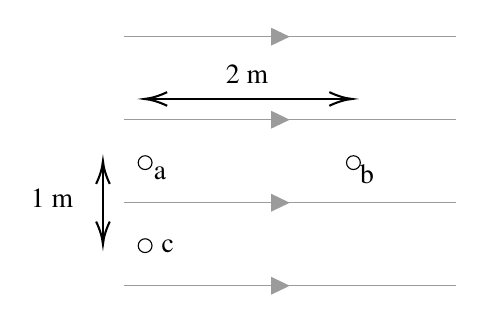
\begin{tikzpicture}[x=0.75pt,y=0.75pt,yscale=-1,xscale=1]
%uncomment if require: \path (0,143); %set diagram left start at 0, and has height of 143

%Straight Lines [id:da884153126551716] 
\draw [color={rgb, 255:red, 155; green, 155; blue, 155 }  ,draw opacity=1 ]   (50,10) -- (210,10) ;
\draw [shift={(130,10)}, rotate = 180] [fill={rgb, 255:red, 155; green, 155; blue, 155 }  ,fill opacity=1 ][line width=0.08]  [draw opacity=0] (8.93,-4.29) -- (0,0) -- (8.93,4.29) -- cycle    ;
%Straight Lines [id:da5466884046634857] 
\draw [color={rgb, 255:red, 155; green, 155; blue, 155 }  ,draw opacity=1 ]   (50,50) -- (210,50) ;
\draw [shift={(130,50)}, rotate = 180] [fill={rgb, 255:red, 155; green, 155; blue, 155 }  ,fill opacity=1 ][line width=0.08]  [draw opacity=0] (8.93,-4.29) -- (0,0) -- (8.93,4.29) -- cycle    ;
%Straight Lines [id:da4563738244773976] 
\draw [color={rgb, 255:red, 155; green, 155; blue, 155 }  ,draw opacity=1 ]   (50,90) -- (210,90) ;
\draw [shift={(130,90)}, rotate = 180] [fill={rgb, 255:red, 155; green, 155; blue, 155 }  ,fill opacity=1 ][line width=0.08]  [draw opacity=0] (8.93,-4.29) -- (0,0) -- (8.93,4.29) -- cycle    ;
%Straight Lines [id:da8861553808606357] 
\draw [color={rgb, 255:red, 155; green, 155; blue, 155 }  ,draw opacity=1 ]   (50,130) -- (210,130) ;
\draw [shift={(130,130)}, rotate = 180] [fill={rgb, 255:red, 155; green, 155; blue, 155 }  ,fill opacity=1 ][line width=0.08]  [draw opacity=0] (8.93,-4.29) -- (0,0) -- (8.93,4.29) -- cycle    ;
%Shape: Circle [id:dp8574197652931845] 
\draw   (63.64,70.68) .. controls (63.64,68.84) and (62.16,67.36) .. (60.32,67.36) .. controls (58.49,67.36) and (57,68.84) .. (57,70.68) .. controls (57,72.51) and (58.49,74) .. (60.32,74) .. controls (62.16,74) and (63.64,72.51) .. (63.64,70.68) -- cycle ;
%Shape: Circle [id:dp7947666583659698] 
\draw   (164,70.68) .. controls (164,68.84) and (162.51,67.36) .. (160.68,67.36) .. controls (158.84,67.36) and (157.36,68.84) .. (157.36,70.68) .. controls (157.36,72.51) and (158.84,74) .. (160.68,74) .. controls (162.51,74) and (164,72.51) .. (164,70.68) -- cycle ;
%Shape: Circle [id:dp6086807902184315] 
\draw   (63.64,110.68) .. controls (63.64,108.84) and (62.16,107.36) .. (60.32,107.36) .. controls (58.49,107.36) and (57,108.84) .. (57,110.68) .. controls (57,112.51) and (58.49,114) .. (60.32,114) .. controls (62.16,114) and (63.64,112.51) .. (63.64,110.68) -- cycle ;
%Straight Lines [id:da08881059573320749] 
\draw    (40,72) -- (40,108) ;
\draw [shift={(40,110)}, rotate = 270] [color={rgb, 255:red, 0; green, 0; blue, 0 }  ][line width=0.75]    (10.93,-3.29) .. controls (6.95,-1.4) and (3.31,-0.3) .. (0,0) .. controls (3.31,0.3) and (6.95,1.4) .. (10.93,3.29)   ;
\draw [shift={(40,70)}, rotate = 90] [color={rgb, 255:red, 0; green, 0; blue, 0 }  ][line width=0.75]    (10.93,-3.29) .. controls (6.95,-1.4) and (3.31,-0.3) .. (0,0) .. controls (3.31,0.3) and (6.95,1.4) .. (10.93,3.29)   ;
%Straight Lines [id:da714465645858051] 
\draw    (158,40) -- (62,40) ;
\draw [shift={(60,40)}, rotate = 360] [color={rgb, 255:red, 0; green, 0; blue, 0 }  ][line width=0.75]    (10.93,-3.29) .. controls (6.95,-1.4) and (3.31,-0.3) .. (0,0) .. controls (3.31,0.3) and (6.95,1.4) .. (10.93,3.29)   ;
\draw [shift={(160,40)}, rotate = 180] [color={rgb, 255:red, 0; green, 0; blue, 0 }  ][line width=0.75]    (10.93,-3.29) .. controls (6.95,-1.4) and (3.31,-0.3) .. (0,0) .. controls (3.31,0.3) and (6.95,1.4) .. (10.93,3.29)   ;

% Text Node
\draw (63.32,71.36) node [anchor=north west][inner sep=0.75pt]   [align=left] {{\fontfamily{ptm}\selectfont a}};
% Text Node
\draw (162.68,70.36) node [anchor=north west][inner sep=0.75pt]   [align=left] {{\fontfamily{ptm}\selectfont b}};
% Text Node
\draw (67,106.68) node [anchor=north west][inner sep=0.75pt]   [align=left] {{\fontfamily{ptm}\selectfont c}};
% Text Node
\draw (4,82) node [anchor=north west][inner sep=0.75pt]   [align=left] {{\fontfamily{ptm}\selectfont 1 m}};
% Text Node
\draw (98,22) node [anchor=north west][inner sep=0.75pt]   [align=left] {{\fontfamily{ptm}\selectfont 2 m}};


\end{tikzpicture}


\begin{enumerate}

  \item A charge of $+3\text{ C}$ is placed at point $A$. What happens to that charge when it is released from rest?

        \ifsolutions
        {\bf Answer}: Moves to right. By convention, electric field lines point in the direction of the force on a positive charge.
        \else

        \vskip 36pt
        \fi

  \item A charge of $+3\text{ C}$ is moved from $A$ to $B$. (a) How much work was done by the electric field? (b) By how much has the potential energy of the charge changed?

        \ifsolutions
        {\bf Answer}: The charge naturally wants to move from $A$ to $B$ because it is a positive charge, and the field line direction indicates the direction of the force on a positive charge. The force the field exerts on the charge is $\bfvec{F}=Q\bfvec{E}=(3\text{ C})(3\text { N/C})\ihat = (9\text{ N})\ihat$, where $\ihat$ points to the right.

        (a) $W=+|\bfvec{F}|L=+(9 \text{ N})(2\text { m})=+18\text{ J}$, and (b) $\Delta U = -18\text{ J}$ (the change in PE, $\Delta U$, is equal and opposite to the work done by the field).
        \else

        \vskip 36pt
        \fi

  \item A charge of $-3\text{ C}$ is placed at point $A$. What happens to that charge when it is released from rest?

        \ifsolutions
        {\bf Answer}: Moves to left.
        \else

        \vskip 48pt
        \fi

  \item A charge of $-3\text{ C}$ is moved from $A$ to $B$. (a) How much work was done by the electric field? (b) By how much has the potential energy of the charge changed?

        \ifsolutions
        {\bf Answer}: (a) $-18\text{ J}$, and (b) $\Delta U = +18\text{ J}$ (the change in PE, $\Delta U$, is equal and opposite to the work done by the field).
        \else

        \vskip 48pt
        \fi

  \item A charge of $-3\text{ C}$ is moved straight downward from $A$ to $D$. (a) How much work was done by the electric field? (b) By how much has the potential energy of the charge changed?

        \ifsolutions
        {\bf Answer}: The force due to the field is always perpendicular to the direction of movement. So the work done is zero: (a) $0\text{ J}$; (b) $0 \text{ J}$.
        \else

        \vskip 48pt
        \fi

  \item If a charge of $-3\text{ C}$ is moved from $A$ to $D$ on a path that is not a straight line, will your answers to the previous problem change? If no, explain why. If yes, provide new answers.

        \ifsolutions
        {\bf Answer}: No, they won't change. Think of movement along a smooth and curved line as being made of a series of tiny and equal-sized steps in vertical and horizontal directions. There is no work associated with the vertical steps. There is positive work associated with steps to the right and negative work associated with steps to the left. To get from $A$ to $D$ along an arbitrary path, you must take an equal number of steps to the left and to the right. See also Figure 23.1 and 23.2 in the textbook, which describes how the work done by a conservative force does not depend on the path.
        \else

        \vskip 36pt
        \fi

\end{enumerate}

\newpage

\subsection{Problem -- Radial Field}

In the previous problem, a charge was moved in a region of space where the electric field was constant and so the calculation of work did not require integration. In this problem, the electric field is not constant and so integration is required. The integration that must be performed to compute work in this case is given by Equation 23.8 in the textbook.



\tikzset{every picture/.style={line width=0.75pt}} %set default line width to 0.75pt        

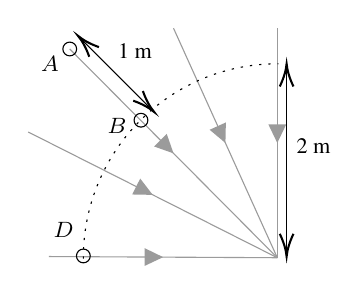
\begin{tikzpicture}[x=0.75pt,y=0.75pt,yscale=-1,xscale=1]
%uncomment if require: \path (0,123); %set diagram left start at 0, and has height of 123

%Straight Lines [id:da7230172572117657] 
\draw [color={rgb, 255:red, 155; green, 155; blue, 155 }  ,draw opacity=1 ]   (130,0) -- (130,110.57) ;
\draw [shift={(130,55.29)}, rotate = 270] [fill={rgb, 255:red, 155; green, 155; blue, 155 }  ,fill opacity=1 ][line width=0.08]  [draw opacity=0] (8.93,-4.29) -- (0,0) -- (8.93,4.29) -- cycle    ;
%Straight Lines [id:da8462561471074679] 
\draw [color={rgb, 255:red, 155; green, 155; blue, 155 }  ,draw opacity=1 ]   (30,10) -- (130,110.57) ;
\draw [shift={(80,60.29)}, rotate = 225.16] [fill={rgb, 255:red, 155; green, 155; blue, 155 }  ,fill opacity=1 ][line width=0.08]  [draw opacity=0] (8.93,-4.29) -- (0,0) -- (8.93,4.29) -- cycle    ;
%Straight Lines [id:da44636059737074385] 
\draw [color={rgb, 255:red, 155; green, 155; blue, 155 }  ,draw opacity=1 ]   (20,110) -- (130,110.57) ;
\draw [shift={(75,110.29)}, rotate = 180.3] [fill={rgb, 255:red, 155; green, 155; blue, 155 }  ,fill opacity=1 ][line width=0.08]  [draw opacity=0] (8.93,-4.29) -- (0,0) -- (8.93,4.29) -- cycle    ;
%Shape: Circle [id:dp15963035926201297] 
\draw   (33.32,10) .. controls (33.32,8.17) and (31.83,6.68) .. (30,6.68) .. controls (28.17,6.68) and (26.68,8.17) .. (26.68,10) .. controls (26.68,11.83) and (28.17,13.32) .. (30,13.32) .. controls (31.83,13.32) and (33.32,11.83) .. (33.32,10) -- cycle ;
%Shape: Circle [id:dp28068496159525824] 
\draw   (67.64,44.32) .. controls (67.64,42.49) and (66.16,41) .. (64.32,41) .. controls (62.49,41) and (61,42.49) .. (61,44.32) .. controls (61,46.16) and (62.49,47.64) .. (64.32,47.64) .. controls (66.16,47.64) and (67.64,46.16) .. (67.64,44.32) -- cycle ;
%Straight Lines [id:da19683913764909322] 
\draw [color={rgb, 255:red, 155; green, 155; blue, 155 }  ,draw opacity=1 ]   (80,0) -- (130,110.57) ;
\draw [shift={(105,55.29)}, rotate = 245.67] [fill={rgb, 255:red, 155; green, 155; blue, 155 }  ,fill opacity=1 ][line width=0.08]  [draw opacity=0] (8.93,-4.29) -- (0,0) -- (8.93,4.29) -- cycle    ;
%Straight Lines [id:da7685850493129691] 
\draw [color={rgb, 255:red, 155; green, 155; blue, 155 }  ,draw opacity=1 ]   (10,50) -- (130,110.57) ;
\draw [shift={(70,80.29)}, rotate = 206.78] [fill={rgb, 255:red, 155; green, 155; blue, 155 }  ,fill opacity=1 ][line width=0.08]  [draw opacity=0] (8.93,-4.29) -- (0,0) -- (8.93,4.29) -- cycle    ;
%Shape: Arc [id:dp5908376434320564] 
\draw  [draw opacity=0][dash pattern={on 0.84pt off 2.51pt}] (36.56,111.03) .. controls (36.45,90.33) and (43.18,69.46) .. (57.15,52.06) .. controls (75.7,28.96) and (102.99,17.01) .. (130.49,17.13) -- (130,110.57) -- cycle ; \draw  [dash pattern={on 0.84pt off 2.51pt}] (36.56,111.03) .. controls (36.45,90.33) and (43.18,69.46) .. (57.15,52.06) .. controls (75.7,28.96) and (102.99,17.01) .. (130.49,17.13) ;  
%Shape: Circle [id:dp41740563202607595] 
\draw   (39.88,109.71) .. controls (39.88,107.88) and (38.39,106.39) .. (36.56,106.39) .. controls (34.72,106.39) and (33.24,107.88) .. (33.24,109.71) .. controls (33.24,111.54) and (34.72,113.03) .. (36.56,113.03) .. controls (38.39,113.03) and (39.88,111.54) .. (39.88,109.71) -- cycle ;
%Straight Lines [id:da7016101246826805] 
\draw    (134.49,108) -- (134.49,19.13) ;
\draw [shift={(134.49,17.13)}, rotate = 90] [color={rgb, 255:red, 0; green, 0; blue, 0 }  ][line width=0.75]    (10.93,-3.29) .. controls (6.95,-1.4) and (3.31,-0.3) .. (0,0) .. controls (3.31,0.3) and (6.95,1.4) .. (10.93,3.29)   ;
\draw [shift={(134.49,110)}, rotate = 270] [color={rgb, 255:red, 0; green, 0; blue, 0 }  ][line width=0.75]    (10.93,-3.29) .. controls (6.95,-1.4) and (3.31,-0.3) .. (0,0) .. controls (3.31,0.3) and (6.95,1.4) .. (10.93,3.29)   ;
%Straight Lines [id:da19280730565536208] 
\draw    (69.23,38.91) -- (35.41,5.09) ;
\draw [shift={(34,3.68)}, rotate = 45] [color={rgb, 255:red, 0; green, 0; blue, 0 }  ][line width=0.75]    (10.93,-3.29) .. controls (6.95,-1.4) and (3.31,-0.3) .. (0,0) .. controls (3.31,0.3) and (6.95,1.4) .. (10.93,3.29)   ;
\draw [shift={(70.64,40.32)}, rotate = 225] [color={rgb, 255:red, 0; green, 0; blue, 0 }  ][line width=0.75]    (10.93,-3.29) .. controls (6.95,-1.4) and (3.31,-0.3) .. (0,0) .. controls (3.31,0.3) and (6.95,1.4) .. (10.93,3.29)   ;

% Text Node
\draw (138,52) node [anchor=north west][inner sep=0.75pt]   [align=left] {{\fontfamily{ptm}\selectfont {\footnotesize 2 m}}};
% Text Node
\draw (52,6) node [anchor=north west][inner sep=0.75pt]   [align=left] {{\fontfamily{ptm}\selectfont {\footnotesize 1 m}}};
% Text Node
\draw (15,12.4) node [anchor=north west][inner sep=0.75pt]  [font=\footnotesize]  {$A$};
% Text Node
\draw (47,42.4) node [anchor=north west][inner sep=0.75pt]  [font=\footnotesize]  {$B$};
% Text Node
\draw (21,92.4) node [anchor=north west][inner sep=0.75pt]  [font=\footnotesize]  {$D$};


\end{tikzpicture}


There is a charge of $-6\text{ C}$ at the origin. Some electric field lines for this charge are shown. To simplify the calculations, use $k=9\cdot 10^9\text{ N}\cdot \text{m}^2/\text{C}^2$.

\begin{enumerate}

  \item A charge of $+3\text{ C}$ is moved from $A$ to $B$. (a) How much work was done by the electric field? (b) By how much has the potential energy of the moved charge changed?

        \ifsolutions
        {\bf Answer}: According to equation 23.8, the work done by the field, labeled $W^E$ here, when a charge $q_0$ is moved from a distance $r_a$ to a distance $r_b$ from a charge $q$ is

        $$
        W^E_{a\rightarrow b} = kqq_o\left(\frac{1}{r_a}-\frac{1}{r_b}\right)
        $$

        For this problem, $q=-6\text{ C}$, $q_0=3\text{ C}$, $r_a=3\text{ m}$, and $r_b=2\text{ m}$.

        $$
        W^E_{a\rightarrow b} = (9\cdot 10^9)(-6)(+3)\left(\frac{1}{3}-\frac{1}{2}\right)\text{ J} = +27\cdot 10^9\text{ J}
        $$

        This is the answer for (a). Note that the work is positive as expected -- the force of the electric field on the charge is in the same direction as its movement. The change in electric potential energy is equal to and opposite of the work done by the field, so (b) $-27\cdot 10^9\text{ J}$. Note that the answer of $27\cdot 10^9\text{ J}$ is unphysically large; it is the amount of energy that you would need to lift $27\cdot 10^9\text{ kg}$ (about $5$ million elephants) by $1\text{ m}$. 
        \else

        \vskip 48pt
        \fi

  \item A charge of $-3\text{ C}$ is moved from $A$ to $B$. (a) How much work was done by the electric field? (b) By how much has the potential energy of the moved charge changed?

        \ifsolutions
        {\bf Answer}: (a) $-27\cdot 10^9\text{ J}$, (b) $+27\cdot 10^9\text{ J}$. 
        \else

        \vskip 48pt
        \fi

  \item A charge of $-3\text{ C}$ is moved from $B$ to $D$ along the dotted curve. (a) How much work was done by the electric field? (b) By how much has the potential energy of the moved charge changed?

        \ifsolutions
        {\bf Answer}: (a) $0\text{ J}$, (b) $0\text{ J}$
        \else

        \vskip 48pt
        \fi

  \item A charge of $-3\text{ C}$ is moved from from $D$ to $B$ but along a path that deviates from the dotted curve. (a) How much work was done by the electric field? (b) By how much has the potential energy of the moved charge changed?

        \ifsolutions
        {\bf Answer}: (a) $0\text{ J}$, (b) $0\text{ J}$
        \fi

\end{enumerate}

\newpage

\section{Electric potential difference, $\Delta V$}

In the previous section, we considered moving an arbitrary amount of charge (either positive or negative) from point $a$ to point $b$ and computed its change in potential energy $\Delta U$.

An electric potential difference $\Delta V$ is defined to be the change in electric potential energy of a test charge, $q_o$ when it is moved from point $a$ to point $b$ divided by $q_o$.

As a result, the only difference between the $\Delta U$ calculations performed previously and $\Delta V$ calculations is that we first compute $\Delta U$ for a $+1\text{ C}$ charge. To get $\Delta V$, we simply divide by $\Delta U$ by $+1\text{ C}$.

The definition of electric potential is similar to the definition of the electric field in that they both involve consideration of a test charge. That is, the electric field is the force on a test charge divided by the magnitude of the test charge:

$$\bfvec{E} = {\bfvec{F}}/{q_o}$$

A change in electric potential is the change in electric potential energy of a positive test charge divided by the magnitude of the test charge's charge:

$$\Delta V = {\Delta U}/{q_o}$$

The advantage of using changes in electric potential ($\Delta V$) as opposed to changes in electric potential energy ($\Delta U$) of a specific amount of charge is that once the electric potential difference $\Delta V$ between two points is known for a test charge, the change in potential energy for an arbitrary amount of charge $Q$ can be computed by simply multiplying $\Delta V$ by $Q$. This is similar to the advantage of the electric field. If we know the electric field at a given point, we can find the force on an arbitrary charge $Q$ at that point by multiplying $\bfvec{E}$ by $Q$.

\newpage

\subsection{Problem}

The following diagram shows a region of space where the electric field is constant and has a value of $3$~N/C. 



\tikzset{every picture/.style={line width=0.75pt}} %set default line width to 0.75pt        

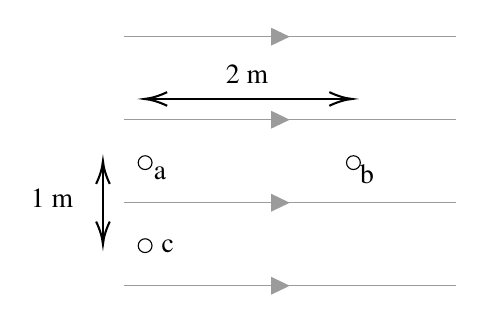
\begin{tikzpicture}[x=0.75pt,y=0.75pt,yscale=-1,xscale=1]
%uncomment if require: \path (0,143); %set diagram left start at 0, and has height of 143

%Straight Lines [id:da884153126551716] 
\draw [color={rgb, 255:red, 155; green, 155; blue, 155 }  ,draw opacity=1 ]   (50,10) -- (210,10) ;
\draw [shift={(130,10)}, rotate = 180] [fill={rgb, 255:red, 155; green, 155; blue, 155 }  ,fill opacity=1 ][line width=0.08]  [draw opacity=0] (8.93,-4.29) -- (0,0) -- (8.93,4.29) -- cycle    ;
%Straight Lines [id:da5466884046634857] 
\draw [color={rgb, 255:red, 155; green, 155; blue, 155 }  ,draw opacity=1 ]   (50,50) -- (210,50) ;
\draw [shift={(130,50)}, rotate = 180] [fill={rgb, 255:red, 155; green, 155; blue, 155 }  ,fill opacity=1 ][line width=0.08]  [draw opacity=0] (8.93,-4.29) -- (0,0) -- (8.93,4.29) -- cycle    ;
%Straight Lines [id:da4563738244773976] 
\draw [color={rgb, 255:red, 155; green, 155; blue, 155 }  ,draw opacity=1 ]   (50,90) -- (210,90) ;
\draw [shift={(130,90)}, rotate = 180] [fill={rgb, 255:red, 155; green, 155; blue, 155 }  ,fill opacity=1 ][line width=0.08]  [draw opacity=0] (8.93,-4.29) -- (0,0) -- (8.93,4.29) -- cycle    ;
%Straight Lines [id:da8861553808606357] 
\draw [color={rgb, 255:red, 155; green, 155; blue, 155 }  ,draw opacity=1 ]   (50,130) -- (210,130) ;
\draw [shift={(130,130)}, rotate = 180] [fill={rgb, 255:red, 155; green, 155; blue, 155 }  ,fill opacity=1 ][line width=0.08]  [draw opacity=0] (8.93,-4.29) -- (0,0) -- (8.93,4.29) -- cycle    ;
%Shape: Circle [id:dp8574197652931845] 
\draw   (63.64,70.68) .. controls (63.64,68.84) and (62.16,67.36) .. (60.32,67.36) .. controls (58.49,67.36) and (57,68.84) .. (57,70.68) .. controls (57,72.51) and (58.49,74) .. (60.32,74) .. controls (62.16,74) and (63.64,72.51) .. (63.64,70.68) -- cycle ;
%Shape: Circle [id:dp7947666583659698] 
\draw   (164,70.68) .. controls (164,68.84) and (162.51,67.36) .. (160.68,67.36) .. controls (158.84,67.36) and (157.36,68.84) .. (157.36,70.68) .. controls (157.36,72.51) and (158.84,74) .. (160.68,74) .. controls (162.51,74) and (164,72.51) .. (164,70.68) -- cycle ;
%Shape: Circle [id:dp6086807902184315] 
\draw   (63.64,110.68) .. controls (63.64,108.84) and (62.16,107.36) .. (60.32,107.36) .. controls (58.49,107.36) and (57,108.84) .. (57,110.68) .. controls (57,112.51) and (58.49,114) .. (60.32,114) .. controls (62.16,114) and (63.64,112.51) .. (63.64,110.68) -- cycle ;
%Straight Lines [id:da08881059573320749] 
\draw    (40,72) -- (40,108) ;
\draw [shift={(40,110)}, rotate = 270] [color={rgb, 255:red, 0; green, 0; blue, 0 }  ][line width=0.75]    (10.93,-3.29) .. controls (6.95,-1.4) and (3.31,-0.3) .. (0,0) .. controls (3.31,0.3) and (6.95,1.4) .. (10.93,3.29)   ;
\draw [shift={(40,70)}, rotate = 90] [color={rgb, 255:red, 0; green, 0; blue, 0 }  ][line width=0.75]    (10.93,-3.29) .. controls (6.95,-1.4) and (3.31,-0.3) .. (0,0) .. controls (3.31,0.3) and (6.95,1.4) .. (10.93,3.29)   ;
%Straight Lines [id:da714465645858051] 
\draw    (158,40) -- (62,40) ;
\draw [shift={(60,40)}, rotate = 360] [color={rgb, 255:red, 0; green, 0; blue, 0 }  ][line width=0.75]    (10.93,-3.29) .. controls (6.95,-1.4) and (3.31,-0.3) .. (0,0) .. controls (3.31,0.3) and (6.95,1.4) .. (10.93,3.29)   ;
\draw [shift={(160,40)}, rotate = 180] [color={rgb, 255:red, 0; green, 0; blue, 0 }  ][line width=0.75]    (10.93,-3.29) .. controls (6.95,-1.4) and (3.31,-0.3) .. (0,0) .. controls (3.31,0.3) and (6.95,1.4) .. (10.93,3.29)   ;

% Text Node
\draw (63.32,71.36) node [anchor=north west][inner sep=0.75pt]   [align=left] {{\fontfamily{ptm}\selectfont a}};
% Text Node
\draw (162.68,70.36) node [anchor=north west][inner sep=0.75pt]   [align=left] {{\fontfamily{ptm}\selectfont b}};
% Text Node
\draw (67,106.68) node [anchor=north west][inner sep=0.75pt]   [align=left] {{\fontfamily{ptm}\selectfont c}};
% Text Node
\draw (4,82) node [anchor=north west][inner sep=0.75pt]   [align=left] {{\fontfamily{ptm}\selectfont 1 m}};
% Text Node
\draw (98,22) node [anchor=north west][inner sep=0.75pt]   [align=left] {{\fontfamily{ptm}\selectfont 2 m}};


\end{tikzpicture}


\begin{enumerate}

  \item What is the difference in electric potential $\Delta V = V_B-V_A$.

        \ifsolutions
        {\bf Answer}: As discussed in the introduction to this section, the difference in electric potential can be determined by first computing $\Delta U$ for a $+1\text{ C}$ charge. Then $\Delta V = \Delta U/(1\text{ C})$. The steps for computing $\Delta V$ for a $+1\text{ C}$ charge will be identical to those in problem 1.1.2 of this tutorial. Using these steps, the result for this problem is $\Delta U=-6\text{ J}$. Thus,

        $$\Delta V = \frac{-6\text{ J}}{+1\text{ C}}= -6\text{ volts}$$

        A faster way of solving this is to simply compute $\Delta V$ by using $\Delta U$ for the $3\text{ C}$ charge considered in 1.1.2 ($-18\text{ J}$) and dividing by $3\text{ C}$. This is also valid and makes sense -- a difference in potential from point $A$ to point $B$ corresponds to the change in potential energy associated with moving a positive unit of charge from point $A$ to point $B$.
        \else

        \vskip 48pt
        \fi

  \item A charge of $+3\text{ C}$ is moved from $A$ to $B$. By how much has the electric potential energy of the moved charge changed?

        \ifsolutions
        {\bf Answer}: This question was already answered previously in 1.1.2. But given $\Delta V$, we can compute $\Delta U$:

        $$\Delta U = Q\Delta V=(3\text{ C})(-6\text{ volt})=(3\text{ C})\left(-6\frac{\text{ J}}{ \text{ C}}\right)=-18\text{ J}$$
        \else

        \vskip 48pt
        \fi

  \item A charge of $-3\text{ C}$ is moved from $A$ to $B$. By how much has the electric potential energy of the moved charge changed?

        \ifsolutions
        {\bf Answer}: This question was already answered previously in 1.1.4. But given $\Delta V$, we can compute $\Delta U$:

        $$
         \Delta U = Q\Delta V=(-3\text{ C})(-6\text{ volt})=(-3\text{ C})\left(-6\frac{\text{ J}}{ \text{ C}}\right)=+18\text{ J}
        $$
        \else

        \vskip 48pt
        \fi

  \item A charge of $-3\text{ C}$ is moved from $B$ to $D$. By how much has the electric potential energy of the moved charge changed?

        \ifsolutions
        {\bf Answer}: The move from $B$ to $D$ can be made by moving from $B$ to $A$ and then moving from $A$ to $D$. The change in potential when moving from $B$ to $A$ is opposite to the change in potential when moving from $A$ to $B$, which was found to be $-6\text{ Volts}$. The change in potential in going from $A$ to $D$ is zero. Thus,

        $$
         \Delta U = Q\Delta V=(-3\text{ C})(+6\text{ volt})=-18\text{ J}
        $$
        \else

        \vskip 48pt
        \fi

  \item What is the difference in electric potential $\Delta V = V_B-V_D$.

        \ifsolutions
        {\bf Answer}: $-6\text{ volt}$. This is the same as $(V_B - V_A) + (V_A - V_D) = -6\text{ volt} + 0 = -6\text{ volt}$
        \else

        \vskip 48pt
        \fi

\end{enumerate}

\newpage

\subsection{Problem}

There is a charge of $-6\text{ C}$ at the origin. Some electric field lines for this charge are shown. To simplify the math, use $k=9\cdot 10^9\text{ N}\cdot\text{m}^2/\text{C}^2$.



\tikzset{every picture/.style={line width=0.75pt}} %set default line width to 0.75pt        

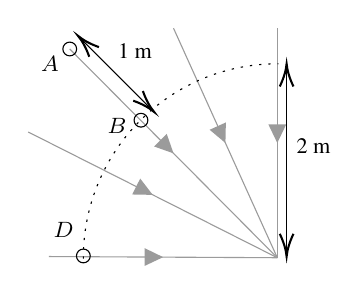
\begin{tikzpicture}[x=0.75pt,y=0.75pt,yscale=-1,xscale=1]
%uncomment if require: \path (0,123); %set diagram left start at 0, and has height of 123

%Straight Lines [id:da7230172572117657] 
\draw [color={rgb, 255:red, 155; green, 155; blue, 155 }  ,draw opacity=1 ]   (130,0) -- (130,110.57) ;
\draw [shift={(130,55.29)}, rotate = 270] [fill={rgb, 255:red, 155; green, 155; blue, 155 }  ,fill opacity=1 ][line width=0.08]  [draw opacity=0] (8.93,-4.29) -- (0,0) -- (8.93,4.29) -- cycle    ;
%Straight Lines [id:da8462561471074679] 
\draw [color={rgb, 255:red, 155; green, 155; blue, 155 }  ,draw opacity=1 ]   (30,10) -- (130,110.57) ;
\draw [shift={(80,60.29)}, rotate = 225.16] [fill={rgb, 255:red, 155; green, 155; blue, 155 }  ,fill opacity=1 ][line width=0.08]  [draw opacity=0] (8.93,-4.29) -- (0,0) -- (8.93,4.29) -- cycle    ;
%Straight Lines [id:da44636059737074385] 
\draw [color={rgb, 255:red, 155; green, 155; blue, 155 }  ,draw opacity=1 ]   (20,110) -- (130,110.57) ;
\draw [shift={(75,110.29)}, rotate = 180.3] [fill={rgb, 255:red, 155; green, 155; blue, 155 }  ,fill opacity=1 ][line width=0.08]  [draw opacity=0] (8.93,-4.29) -- (0,0) -- (8.93,4.29) -- cycle    ;
%Shape: Circle [id:dp15963035926201297] 
\draw   (33.32,10) .. controls (33.32,8.17) and (31.83,6.68) .. (30,6.68) .. controls (28.17,6.68) and (26.68,8.17) .. (26.68,10) .. controls (26.68,11.83) and (28.17,13.32) .. (30,13.32) .. controls (31.83,13.32) and (33.32,11.83) .. (33.32,10) -- cycle ;
%Shape: Circle [id:dp28068496159525824] 
\draw   (67.64,44.32) .. controls (67.64,42.49) and (66.16,41) .. (64.32,41) .. controls (62.49,41) and (61,42.49) .. (61,44.32) .. controls (61,46.16) and (62.49,47.64) .. (64.32,47.64) .. controls (66.16,47.64) and (67.64,46.16) .. (67.64,44.32) -- cycle ;
%Straight Lines [id:da19683913764909322] 
\draw [color={rgb, 255:red, 155; green, 155; blue, 155 }  ,draw opacity=1 ]   (80,0) -- (130,110.57) ;
\draw [shift={(105,55.29)}, rotate = 245.67] [fill={rgb, 255:red, 155; green, 155; blue, 155 }  ,fill opacity=1 ][line width=0.08]  [draw opacity=0] (8.93,-4.29) -- (0,0) -- (8.93,4.29) -- cycle    ;
%Straight Lines [id:da7685850493129691] 
\draw [color={rgb, 255:red, 155; green, 155; blue, 155 }  ,draw opacity=1 ]   (10,50) -- (130,110.57) ;
\draw [shift={(70,80.29)}, rotate = 206.78] [fill={rgb, 255:red, 155; green, 155; blue, 155 }  ,fill opacity=1 ][line width=0.08]  [draw opacity=0] (8.93,-4.29) -- (0,0) -- (8.93,4.29) -- cycle    ;
%Shape: Arc [id:dp5908376434320564] 
\draw  [draw opacity=0][dash pattern={on 0.84pt off 2.51pt}] (36.56,111.03) .. controls (36.45,90.33) and (43.18,69.46) .. (57.15,52.06) .. controls (75.7,28.96) and (102.99,17.01) .. (130.49,17.13) -- (130,110.57) -- cycle ; \draw  [dash pattern={on 0.84pt off 2.51pt}] (36.56,111.03) .. controls (36.45,90.33) and (43.18,69.46) .. (57.15,52.06) .. controls (75.7,28.96) and (102.99,17.01) .. (130.49,17.13) ;  
%Shape: Circle [id:dp41740563202607595] 
\draw   (39.88,109.71) .. controls (39.88,107.88) and (38.39,106.39) .. (36.56,106.39) .. controls (34.72,106.39) and (33.24,107.88) .. (33.24,109.71) .. controls (33.24,111.54) and (34.72,113.03) .. (36.56,113.03) .. controls (38.39,113.03) and (39.88,111.54) .. (39.88,109.71) -- cycle ;
%Straight Lines [id:da7016101246826805] 
\draw    (134.49,108) -- (134.49,19.13) ;
\draw [shift={(134.49,17.13)}, rotate = 90] [color={rgb, 255:red, 0; green, 0; blue, 0 }  ][line width=0.75]    (10.93,-3.29) .. controls (6.95,-1.4) and (3.31,-0.3) .. (0,0) .. controls (3.31,0.3) and (6.95,1.4) .. (10.93,3.29)   ;
\draw [shift={(134.49,110)}, rotate = 270] [color={rgb, 255:red, 0; green, 0; blue, 0 }  ][line width=0.75]    (10.93,-3.29) .. controls (6.95,-1.4) and (3.31,-0.3) .. (0,0) .. controls (3.31,0.3) and (6.95,1.4) .. (10.93,3.29)   ;
%Straight Lines [id:da19280730565536208] 
\draw    (69.23,38.91) -- (35.41,5.09) ;
\draw [shift={(34,3.68)}, rotate = 45] [color={rgb, 255:red, 0; green, 0; blue, 0 }  ][line width=0.75]    (10.93,-3.29) .. controls (6.95,-1.4) and (3.31,-0.3) .. (0,0) .. controls (3.31,0.3) and (6.95,1.4) .. (10.93,3.29)   ;
\draw [shift={(70.64,40.32)}, rotate = 225] [color={rgb, 255:red, 0; green, 0; blue, 0 }  ][line width=0.75]    (10.93,-3.29) .. controls (6.95,-1.4) and (3.31,-0.3) .. (0,0) .. controls (3.31,0.3) and (6.95,1.4) .. (10.93,3.29)   ;

% Text Node
\draw (138,52) node [anchor=north west][inner sep=0.75pt]   [align=left] {{\fontfamily{ptm}\selectfont {\footnotesize 2 m}}};
% Text Node
\draw (52,6) node [anchor=north west][inner sep=0.75pt]   [align=left] {{\fontfamily{ptm}\selectfont {\footnotesize 1 m}}};
% Text Node
\draw (15,12.4) node [anchor=north west][inner sep=0.75pt]  [font=\footnotesize]  {$A$};
% Text Node
\draw (47,42.4) node [anchor=north west][inner sep=0.75pt]  [font=\footnotesize]  {$B$};
% Text Node
\draw (21,92.4) node [anchor=north west][inner sep=0.75pt]  [font=\footnotesize]  {$D$};


\end{tikzpicture}


\begin{enumerate}

  \item What is the difference in potential $\Delta V = V_B-V_A$?

        \ifsolutions
        {\bf Answer}:

        The potential at a point in space due to a point charge $q$ a distance $r$ from that point is $V={kq}/{r}$.

        $$V_A=\frac{k(-6\text{ C})}{3\text { m}}=-18\cdot 10^9\text{ volt}$$

        $$V_B=\frac{k(-6\text{ C})}{2\text { m}}=-27\cdot 10^9\text{ volt}$$

        $$V_B-V_A=-9\cdot 10^9\text{ volt}$$

        A negative value is expected because a positive charge placed at $A$ will tend to move towards $B$, which has a lower potential.
        \else

        \vskip 48pt
        \fi

  \item A charge of $-3\text{ C}$ is moved from $A$ to $B$. By how much has the electric potential energy of the moved charge changed?

        \ifsolutions
        {\bf Answer}:

        This is most easily found using

        $$\Delta U = Q{\Delta V}$$

        From part 1., $V_B-V_A=-9\cdot 10^9\text{ volt}$. As a result, 

        $$U_B-U_A= (-3\text{ C})(V_B-V_A)=+27\cdot 10^9$$

        This answer matches the answer to the identical question of problem 1.1.2.
        \else

        \vskip 48pt
        \fi

  \item Aa charge of $-3\text{ C}$ is moved from $B$ to $D$. By how much has the electric potential energy of the moved charge changed?

        \ifsolutions
        {\bf Answer}: $0\text{ J}$.
        \else

        \vskip 48pt
        \fi

  \item What is difference in electric potential $\Delta V = V_D-V_A$.

        \ifsolutions
        {\bf Answer}: The potential at $D$ is the same as the potential at $B$. This can be seen mathematically from the equation $V=\frac{kq}{r}$ -- at $D$ and $B$, $r$ is the same. Physically, in moving from $B$ to $D$ along the dotted line, no work is required because the electric field is perpendicular to this path. The problem statement did not require moving from $B$ to $D$ along the dotted line, but was established earlier, the changes in potential energy are independent of the path for a conservative force, so we are free to choose a convenient path. Based on this, $V_D-V_A=V_B-V_A$ and so the answer is the same as that for part 1. of this problem: $-9\cdot 10^9\text{ volt}$.
        \else

        \vskip 48pt
        \fi

\end{enumerate}

\newpage

\section{$U$ and $V$ and Superposition}

%Recall that the work done by the electric field when a charge $q_0$ is moved from $a$ to $b$ is

%$$
%W^E_{a\rightarrow b} = kqq_o\left(\frac{1}{r_a}-\frac{1}{r_b}\right)
%$$

%Plugging in $a=\infty$ and $b=r_1$ gives

%$$
%W^E_{\infty\rightarrow r_1}
%= kqq_o\left(\frac{1}{\infty}-\frac{1}{r_1}\right) 
%= -k\frac{q_0q_1}{r_1}
%$$

%$$
%W_{a\rightarrow b}^{
%\text{cons}} \equiv -\Delta U = -(U_b-U_a)
%$$

The electric potential energy of a charge $q_0$ that is a distance of $r_1$ from a charge $q_1$ is defined to be 

$$
U=k\frac{q_0q_1}{r_1}
$$

This corresponds to the work required to move $q_0$ from infinity to $r_1$. 
In this formula, if the charges have opposite signs then $U$ is negative; if they have the same sign then $U$  is positive. Note that there is a sign associated with the potential energy, but the direction of the vector that connects the charges does not matter; the equation for $U$ only involves the values of the charges and the magnitude of the separation distance between them. As a result, we can also state that the formula above corresponds to the work required to move $q_1$ from infinity to a distance $r_1$ from $q_0$.

Consider next the potential energy of charge $q_0$ when it is a distance $r_1$ from charge $q_1$ and a distance $r_2$ from charge $q_2$. The potential energy of $q_0$ is the sum

$$
U=k\frac{q_0q_1}{r_1}+k\frac{q_0q_2}{r_2}
$$

More generally, if $q_o$ is among a group of $N$ other charges, the potential energy of $q_0$ is

$$
U=k q_0 \sum_{i=1}^N {\frac{q_i}{r_i}}
$$

Dividing by $q_o$ gives the electric potential at a point in space due to a group of $N$ charges:

$$
V=k \sum_{i=1}^N {\frac{q_i}{r_i}}
$$

\newpage

\subsection{Problem}



\tikzset{every picture/.style={line width=0.75pt}} %set default line width to 0.75pt        

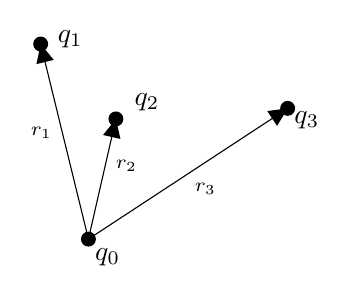
\begin{tikzpicture}[x=0.75pt,y=0.75pt,yscale=-1,xscale=1]
%uncomment if require: \path (0,133); %set diagram left start at 0, and has height of 133

%Shape: Circle [id:dp17890206998831304] 
\draw  [fill={rgb, 255:red, 0; green, 0; blue, 0 }  ,fill opacity=1 ] (42.88,106.71) .. controls (42.88,104.88) and (41.39,103.39) .. (39.56,103.39) .. controls (37.72,103.39) and (36.24,104.88) .. (36.24,106.71) .. controls (36.24,108.54) and (37.72,110.03) .. (39.56,110.03) .. controls (41.39,110.03) and (42.88,108.54) .. (42.88,106.71) -- cycle ;
%Shape: Circle [id:dp6481825116782165] 
\draw  [fill={rgb, 255:red, 0; green, 0; blue, 0 }  ,fill opacity=1 ] (19.88,12.71) .. controls (19.88,10.88) and (18.39,9.39) .. (16.56,9.39) .. controls (14.72,9.39) and (13.24,10.88) .. (13.24,12.71) .. controls (13.24,14.54) and (14.72,16.03) .. (16.56,16.03) .. controls (18.39,16.03) and (19.88,14.54) .. (19.88,12.71) -- cycle ;
%Shape: Circle [id:dp15379389351529782] 
\draw  [fill={rgb, 255:red, 0; green, 0; blue, 0 }  ,fill opacity=1 ] (56.12,48.8) .. controls (56.12,46.97) and (54.63,45.48) .. (52.8,45.48) .. controls (50.97,45.48) and (49.48,46.97) .. (49.48,48.8) .. controls (49.48,50.63) and (50.97,52.12) .. (52.8,52.12) .. controls (54.63,52.12) and (56.12,50.63) .. (56.12,48.8) -- cycle ;
%Shape: Circle [id:dp11075980910893568] 
\draw  [fill={rgb, 255:red, 0; green, 0; blue, 0 }  ,fill opacity=1 ] (138.88,43.71) .. controls (138.88,41.88) and (137.39,40.39) .. (135.56,40.39) .. controls (133.72,40.39) and (132.24,41.88) .. (132.24,43.71) .. controls (132.24,45.54) and (133.72,47.03) .. (135.56,47.03) .. controls (137.39,47.03) and (138.88,45.54) .. (138.88,43.71) -- cycle ;
%Straight Lines [id:da4924768531184569] 
\draw    (39.56,106.71) -- (17.27,15.62) ;
\draw [shift={(16.56,12.71)}, rotate = 76.25] [fill={rgb, 255:red, 0; green, 0; blue, 0 }  ][line width=0.08]  [draw opacity=0] (8.93,-4.29) -- (0,0) -- (8.93,4.29) -- cycle    ;
%Straight Lines [id:da9255120226414246] 
\draw    (39.56,106.71) -- (52.13,51.72) ;
\draw [shift={(52.8,48.8)}, rotate = 102.88] [fill={rgb, 255:red, 0; green, 0; blue, 0 }  ][line width=0.08]  [draw opacity=0] (8.93,-4.29) -- (0,0) -- (8.93,4.29) -- cycle    ;
%Straight Lines [id:da4442580804570828] 
\draw    (39.56,106.71) -- (133.05,45.36) ;
\draw [shift={(135.56,43.71)}, rotate = 146.73] [fill={rgb, 255:red, 0; green, 0; blue, 0 }  ][line width=0.08]  [draw opacity=0] (8.93,-4.29) -- (0,0) -- (8.93,4.29) -- cycle    ;

% Text Node
\draw (41.56,110.11) node [anchor=north west][inner sep=0.75pt]    {$q_{0}$};
% Text Node
\draw (23.56,5.11) node [anchor=north west][inner sep=0.75pt]    {$q_{1}$};
% Text Node
\draw (60.56,35.11) node [anchor=north west][inner sep=0.75pt]    {$q_{2}$};
% Text Node
\draw (137.56,43.79) node [anchor=north west][inner sep=0.75pt]    {$q_{3}$};
% Text Node
\draw (89.56,78.61) node [anchor=north west][inner sep=0.75pt]  [font=\scriptsize]  {$r_{3}$};
% Text Node
\draw (51.56,67.4) node [anchor=north west][inner sep=0.75pt]  [font=\scriptsize]  {$r_{2}$};
% Text Node
\draw (10.56,51.4) node [anchor=north west][inner sep=0.75pt]  [font=\scriptsize]  {$r_{1}$};


\end{tikzpicture}


\begin{enumerate}

  \item What is the electric potential energy of the charge $q_0$ in the diagram shown?

        \ifsolutions
        {\bf Answer}

        $$
        U = \frac{kq_oq_1}{r_1}+\frac{kq_oq_2}{r_2}+\frac{kq_oq_3}{r_3}
        $$

        This represents the amount of energy it would take to move charge $q_o$ from infinity to its position on the 
        diagram.
        \else

        \vskip 48pt
        \fi

  \item What is the electric potential at the position of $q_0$ if $q_0$ was not there?

        \ifsolutions
        {\bf Answer}

        $$
        V = \frac{kq_1}{r_1}+\frac{kq_2}{r_2}+\frac{kq_3}{r_3}
        $$

        %That is, the potential at a given location is found from potential energy of a charge at that location by dividing by the charge's potential energy by the value of the charge.
        \else

        \vskip 48pt
        \fi

  \item Can you find the potential energy at the position of $q_0$ if that charge was not there? Why or why not?

        \ifsolutions
        {\bf Answer}: No. It does not make sense to ask what the potential energy is at a point in space. Only physical objects (e.g., masses, charges) have potential energy.
        \else

        \vskip 48pt
        \fi

  \item Explain the difference between potential and potential energy.

        \ifsolutions
        {\bf Answer}: Potential energy is the energy associated with an object at a given location in space. The electric potential energy of a charge is the energy required to move it from a large distance away from all other charges to a given location in space. The electric potential energy of a charge $Q$ at a point in space is related to the electric potential at that point in space by $U=QV$.
        \else

        \vskip 48pt
        \fi

\end{enumerate}

\newpage

\subsection{Problem}

Given a point charge $q_1$ at the origin:

\begin{enumerate}

  \item Write the general equation for the electric potential at a distance $r$ from $q_1$

        \ifsolutions
        \textbf{Answer}:
        $V=kq_1/r$
        \else

        \vskip 36pt
        \fi

  \item Find the electric potential, $V_1$, at $(x,y) = (-d,0)$ due to $q_1$.

        \ifsolutions
        \textbf{Answer}:
        $V_1(d,0)=kq_1/d$
        \else

        \vskip 36pt
        \fi

  \item If a charge $q_2$ is placed at $(x,y) = (d,0)$, find the electric potential, $V$, at $(x,y) = (-d,0)$ (hint -- it is the sum of the electric potentials at due to $q_1$ and $q_2$).

        \ifsolutions
        \textbf{Answer}:
        $V(-d,0)=V_1(-d,0)+V_2(-d,0) = kq_1/d + kq_2/2d$
        \else

        \vskip 36pt
        \fi

  \item How much work is required to place charge $q_3$ at $(x,y) = (-d,0)$?

        \ifsolutions
        \textbf{Answer}:
        $U=W=q_3V(-d,0)=q_3(kq_1/d + kq_2/2d)$
        \else

        \vskip 36pt
        \fi

  \item What is the potential energy, $U$, of $q_3$ when it is at $(x,y) = (-d,0)$?

        \ifsolutions
        \textbf{Answer}:
        See 4.
        \else

        \vskip 36pt
        \fi

\end{enumerate}

%In summary, to find the work required to put a charge $Q$ at point $P$ (or, equivalently, the electric potential energy $U$ of a single charge $Q$ when it is at point $P$), find the potential $V$ at point $P$ due to all of the other charges and then $U = QV$.

\newpage

\section{Energy to Assemble a Collection of Charges}

In the previous problem you computed the work required to move $q_3$ to $(x,y) = (-d,0)$ after $q_2$ was in place. The total work required to assemble the system of three charges is larger than this work because it also took work to move $q_2$ into place. Given a point charge $q_1$ at origin, as in the previous question,

\begin{enumerate}

  \item how much work is required to move $q_2$ to $(x,y) = (d,0)$?;

        \ifsolutions
        \textbf{Answer}:
        $W = q_2V_1(0,d) = q_2(kq_1/d)$
        \else

        \vskip 36pt
        \fi

  \item how much work is required to move $q_3$ to $(x,y) = (-d,0)$ if only $q_1$ is present?;

        \ifsolutions
        \textbf{Answer}:
        $W = q_3V_1(-d,0) = q_3(kq_1/d)$
        \else

        \vskip 36pt
        \fi

  \item how much work is required to move $q_3$ to $(x,y) = (-d,0)$ if only $q_2$ is present?

        \ifsolutions
        \textbf{Answer}:
        $W=q_3V_2(-d,0)=q_3kq_2/2d$
        \else

        \vskip 36pt
        \fi

  \item The total work required to assemble the system of three charges is the sum of the work from parts 1.-3.. Write the equation for this sum in terms of the given variables. (This sum is known as the total potential energy of the system of charges -- see equation 23.11 of the textbook.)

        \ifsolutions
        \textbf{Answer}:
        $W=q_2kq_1/d +  q_3(kq_1/d) + q_3kq_2/2d$
        \fi

\end{enumerate}

\end{document}